\section{機器人模型}
\label{sec:robot}

\subsection{外觀與尺寸}

模型以「像素」為單位（$1 \text{px} = \frac{1}{16} \text{公尺}$），
機器人高 28 px、寬 14 px、厚 5 px（1.75 $\times$ 0.875 $\times$ 0.3125 公尺），
由頭、脖子、軀幹與左右上臂、前臂、大腿、小腿共 11 個部位組成（圖~\ref{fig:robot-look}）。
各部位的局部坐標系（LCS）原點設在關節上，$+y$ 朝上、$+z$ 朝前、$+x$ 朝左。

\begin{figure}[htbp]
    \centering
    \begin{subfigure}[t]{.32\textwidth}
        \centering
        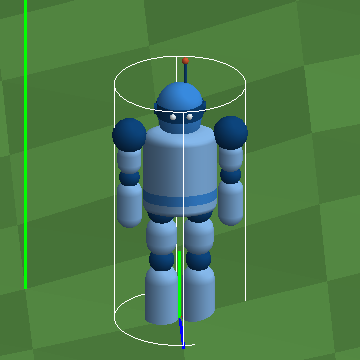
\includegraphics[width=\linewidth]{docs/figures/hw2/ch03_robot-front.png}
        \caption{正面}
    \end{subfigure}\hfill
    \begin{subfigure}[t]{.32\textwidth}
        \centering
        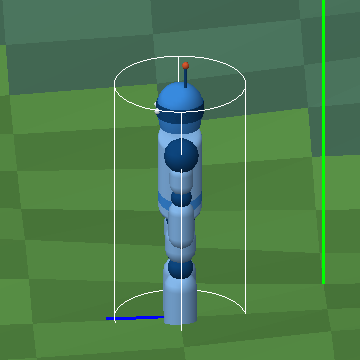
\includegraphics[width=\linewidth]{docs/figures/hw2/ch03_robot-side.png}
        \caption{側面}
    \end{subfigure}\hfill
    \begin{subfigure}[t]{.32\textwidth}
        \centering
        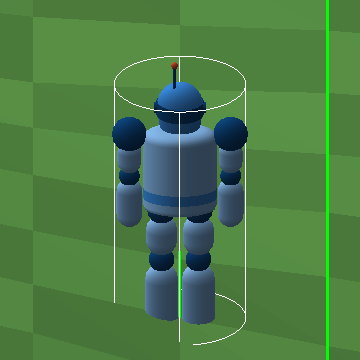
\includegraphics[width=\linewidth]{docs/figures/hw2/ch03_robot-back.png}
        \caption{背面}
    \end{subfigure}
    \caption{機器人的外觀}
    \label{fig:robot-look}
\end{figure}

每個部位都是三角形網格：先用直線、圓弧與 Bézier 曲線在 $x$-$y$ 平面畫出 2D 剖面，
再由 \lstinline|MeshBuilder| 繞 $y$ 軸旋轉成旋轉體（lathe）。

由於純色模型看不出立體表面，因此我參考 Inigo Quilez 的作法，依法向量 $\mathbf{n}$ 與太陽方向 $\mathbf{l}$ 調整亮度。
$\max(0, \mathbf{n} \cdot \mathbf{l})$ 會讓背光面全部同樣暗，所以改將內積映射到 $[0, 1]$ 後平方：
$$
    b(\mathbf{n}) = \left( \tfrac{1}{2}\, \mathbf{n} \cdot \mathbf{l} + \tfrac{1}{2} \right)^2, \qquad
    s(\mathbf{n}) = \min\!\left( 1,\; 0.32 + 0.68 \times 0.9 \times \frac{b(\mathbf{n})}{b(\hat{\mathbf{y}})} \right).
$$
倍率 $s$ 下限為 0.32，避免背光面全黑；平地（$\mathbf{n} = \hat{\mathbf{y}}$）校正為 0.9，讓朝向太陽的斜面仍比平地亮。


\subsection{場景圖}
\label{sec:scene-graph}

機器人的場景圖如圖~\ref{fig:scene-graph}。
每個節點是一根骨頭（bone），記錄它的父節點、關節在父節點座標系中的位置（pivot），以及可轉動的角度範圍。
根節點 root 本身沒有關節，只帶有一個隨姿勢改變的平移量 rootOffset，用來決定髖部離地的高度。
軀幹的原點在髖部中央，雙腿從髖部往下、雙臂從肩膀往下延伸，脖子接在軀幹頂端，頭再接在脖子上。

\begin{figure}[htbp]
    \centering
    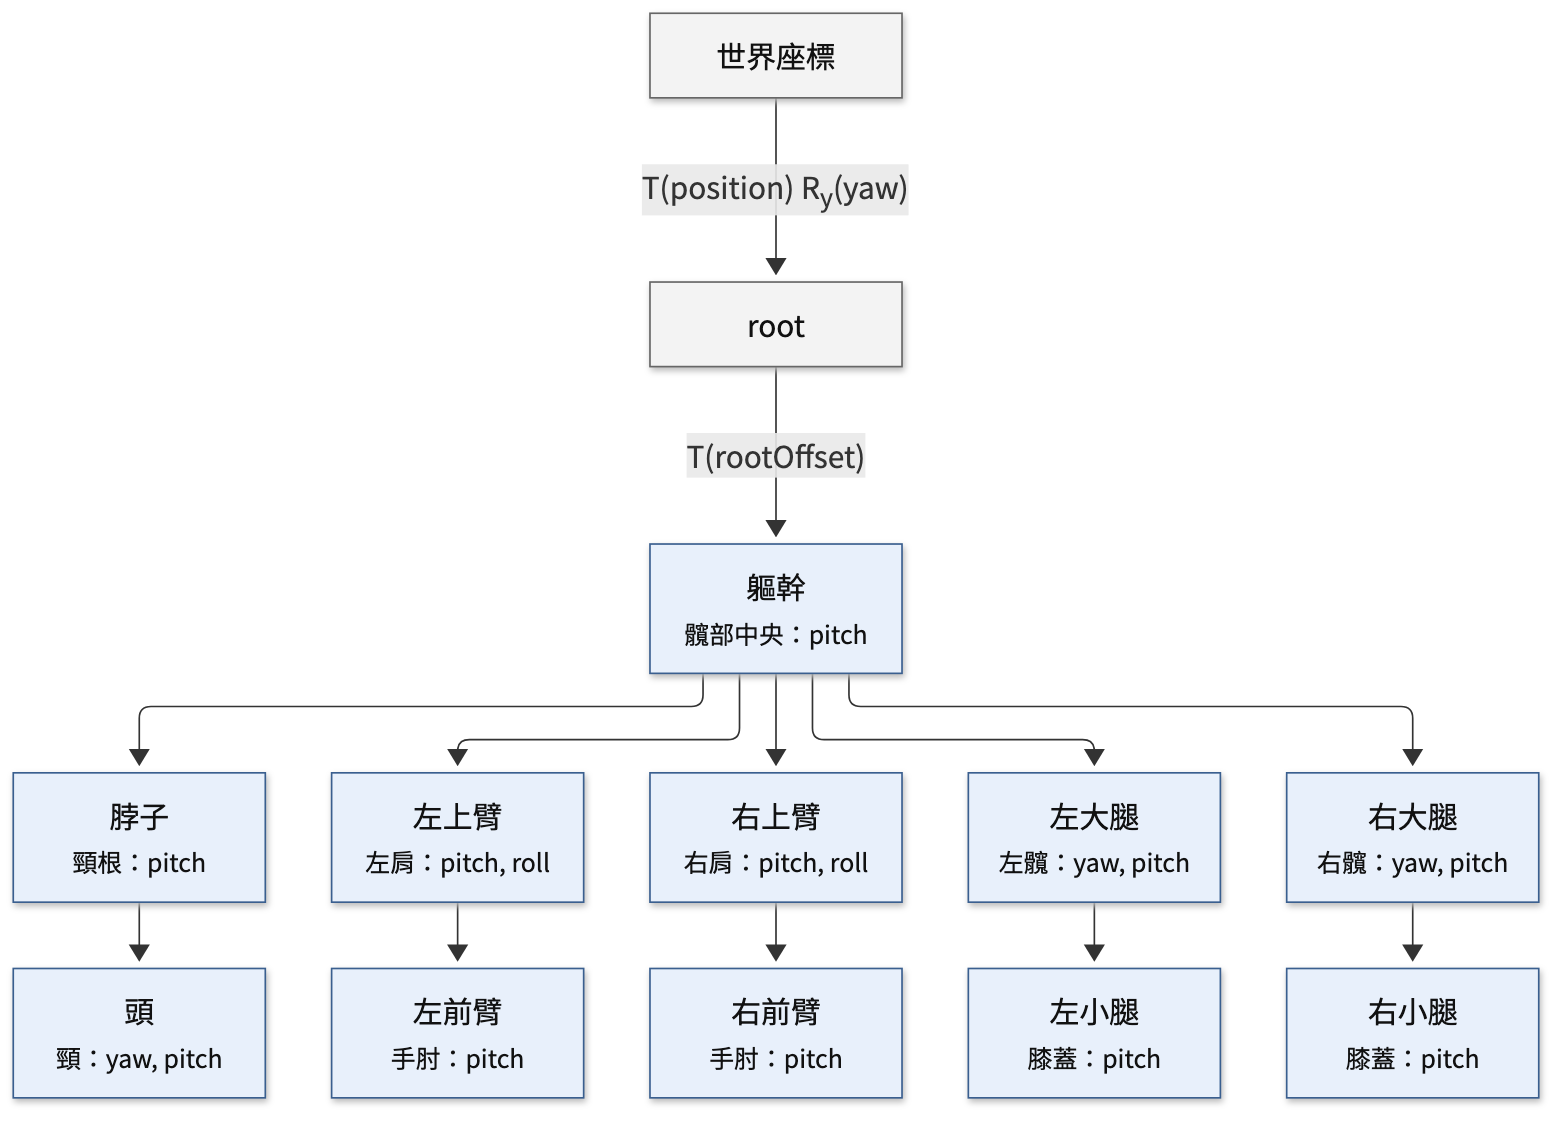
\includegraphics[width=.8\textwidth]{docs/figures/hw2/ch03_scene-graph.png}
    \caption{機器人的場景圖，節點下方為連接父節點的關節與其可轉動的軸}
    \label{fig:scene-graph}
\end{figure}

\subsection{關節自由度}
\label{sec:dof}

每個關節最多有 yaw（繞 $y$ 軸）、pitch（繞 $-x$ 軸）、roll（繞 $z$ 軸）三個旋轉自由度；角度範圍上下限相同的軸視為鎖住，不算一個自由度。
骨頭在靜止姿勢時面向 $+z$，pitch 取 $-x$ 為轉軸，正值就是往前抬起，與視線的 pitch 方向一致。
各關節的自由度與角度範圍如表~\ref{tab:dof}，角度範圍以左側為準，右側的 yaw 與 roll 範圍左右對稱、正負相反。
四肢共有 12 個自由度，加上軀幹、脖子各 1 個與頭部的 2 個，機器人身上共有 16 個旋轉自由度；
另外整隻機器人在世界中還有位置 $(x, y, z)$ 與朝向 yaw 共 4 個自由度。

\begin{table}[H]
    \centering
    \caption{關節的自由度與角度範圍（「—」表示鎖住）}
    \label{tab:dof}
    \small
    \begin{tabular}{lcccc}
        \toprule
        關節       & yaw                       & pitch                      & roll                     & 自由度 \\
        \midrule
        軀幹（髖部中央） & —                         & $-45^\circ \sim 45^\circ$  & —                        & 1   \\
        脖子（頸根）   & —                         & $-45^\circ \sim 45^\circ$  & —                        & 1   \\
        頭（頸）     & $-70^\circ \sim 70^\circ$ & $-60^\circ \sim 50^\circ$  & —                        & 2   \\
        上臂（肩膀）×2 & —                         & $-60^\circ \sim 200^\circ$ & $0^\circ \sim 170^\circ$ & 2   \\
        前臂（手肘）×2 & —                         & $0^\circ \sim 145^\circ$   & —                        & 1   \\
        大腿（髖）×2  & $0^\circ \sim 45^\circ$   & $-30^\circ \sim 120^\circ$ & —                        & 2   \\
        小腿（膝蓋）×2 & —                         & $-140^\circ \sim 0^\circ$  & —                        & 1   \\
        \bottomrule
    \end{tabular}
\end{table}

\subsection{階層繪製}

階層模型的變換順序是先移到關節位置，再套用關節旋轉；所有子節點都會繼承這個變換。
程式用相同順序計算骨頭 $i$ 在機器人模型空間中的矩陣 $M_i$：
$$
    \begin{cases}
        M_{\text{root}} = M_0 = T(\text{rootOffset}), \\
        M_i = M_{\text{parent}(i)} T(\text{pivot}_i)
        R_y(\text{yaw}_i) R_{-x}(\text{pitch}_i) R_z(\text{roll}_i), i \neq \text{root}.
    \end{cases}
$$
骨頭依加入順序儲存，而且父節點一定在子節點之前，因此從頭走過陣列一次就能算完所有矩陣，不需要遞迴。
計算矩陣前，各角度會先限制在表~\ref{tab:dof} 的範圍內，避免姿勢與動畫疊加後超出關節活動範圍。

繪製時先以 \lstinline|glTranslatef|、\lstinline|glRotatef| 移到機器人的位置與朝向，
再對每根骨頭 \lstinline|glPushMatrix|、\lstinline|glMultMatrixf(|$M_i$\lstinline|)|、畫出網格、\lstinline|glPopMatrix|。
由於矩陣採用 OpenGL 的 column-major 排列，可以直接交給 \lstinline|glMultMatrixf|。

這組矩陣也不只用於繪圖。例如，當機器人位於 $\mathbf{p}$、朝向 $\psi$ 時，頭部上的眼睛標記點可由
$$
    \mathbf{p}_{\text{eye,world}} = T(\mathbf{p})R_y(\psi)M_{\text{head}}
    \begin{bmatrix}\mathbf{p}_{\text{eye,local}}\\1\end{bmatrix}
$$
轉成世界座標，作為相機的焦點。
